% Copied from DESTION paper
The BriefCASE environment provides systems engineers with a workflow and tool support for developing
products with inherent cyber-resiliency. 

The  workflow starts with the development of a baseline AADL model of the system architecture
focusing on the desired functionality. This model can be analyzed using any of the existing AADL 
tools (e.g., resource usage, information flow, latency) to determine whether it is acceptable.
BriefCASE integrates additional tools that analyze the architecture model for cybersecurity vulnerabilities and
generate requirements that, when addressed, will mitigate those vulnerabilities.
These requirements are imported into the model and may be addressed using a 
collection of automated model transforms. As requirements are addressed in the design, an assurance case is updated with
corresponding evidence, computed directly from the model or by supporting analysis tools.  
Code implementing new high-assurance components as well as communication and execution infrastructure
is generated from the model along with associated assurance evidence.  

The BriefCASE tools and their interactions are shown in \figref{fig:tool-arch}.   
The following sections describe each step of the workflow in more detail, corresponding
to the tools and artifacts shown in green in the figure.  

\begin{figure*}
	\begin{center}
	  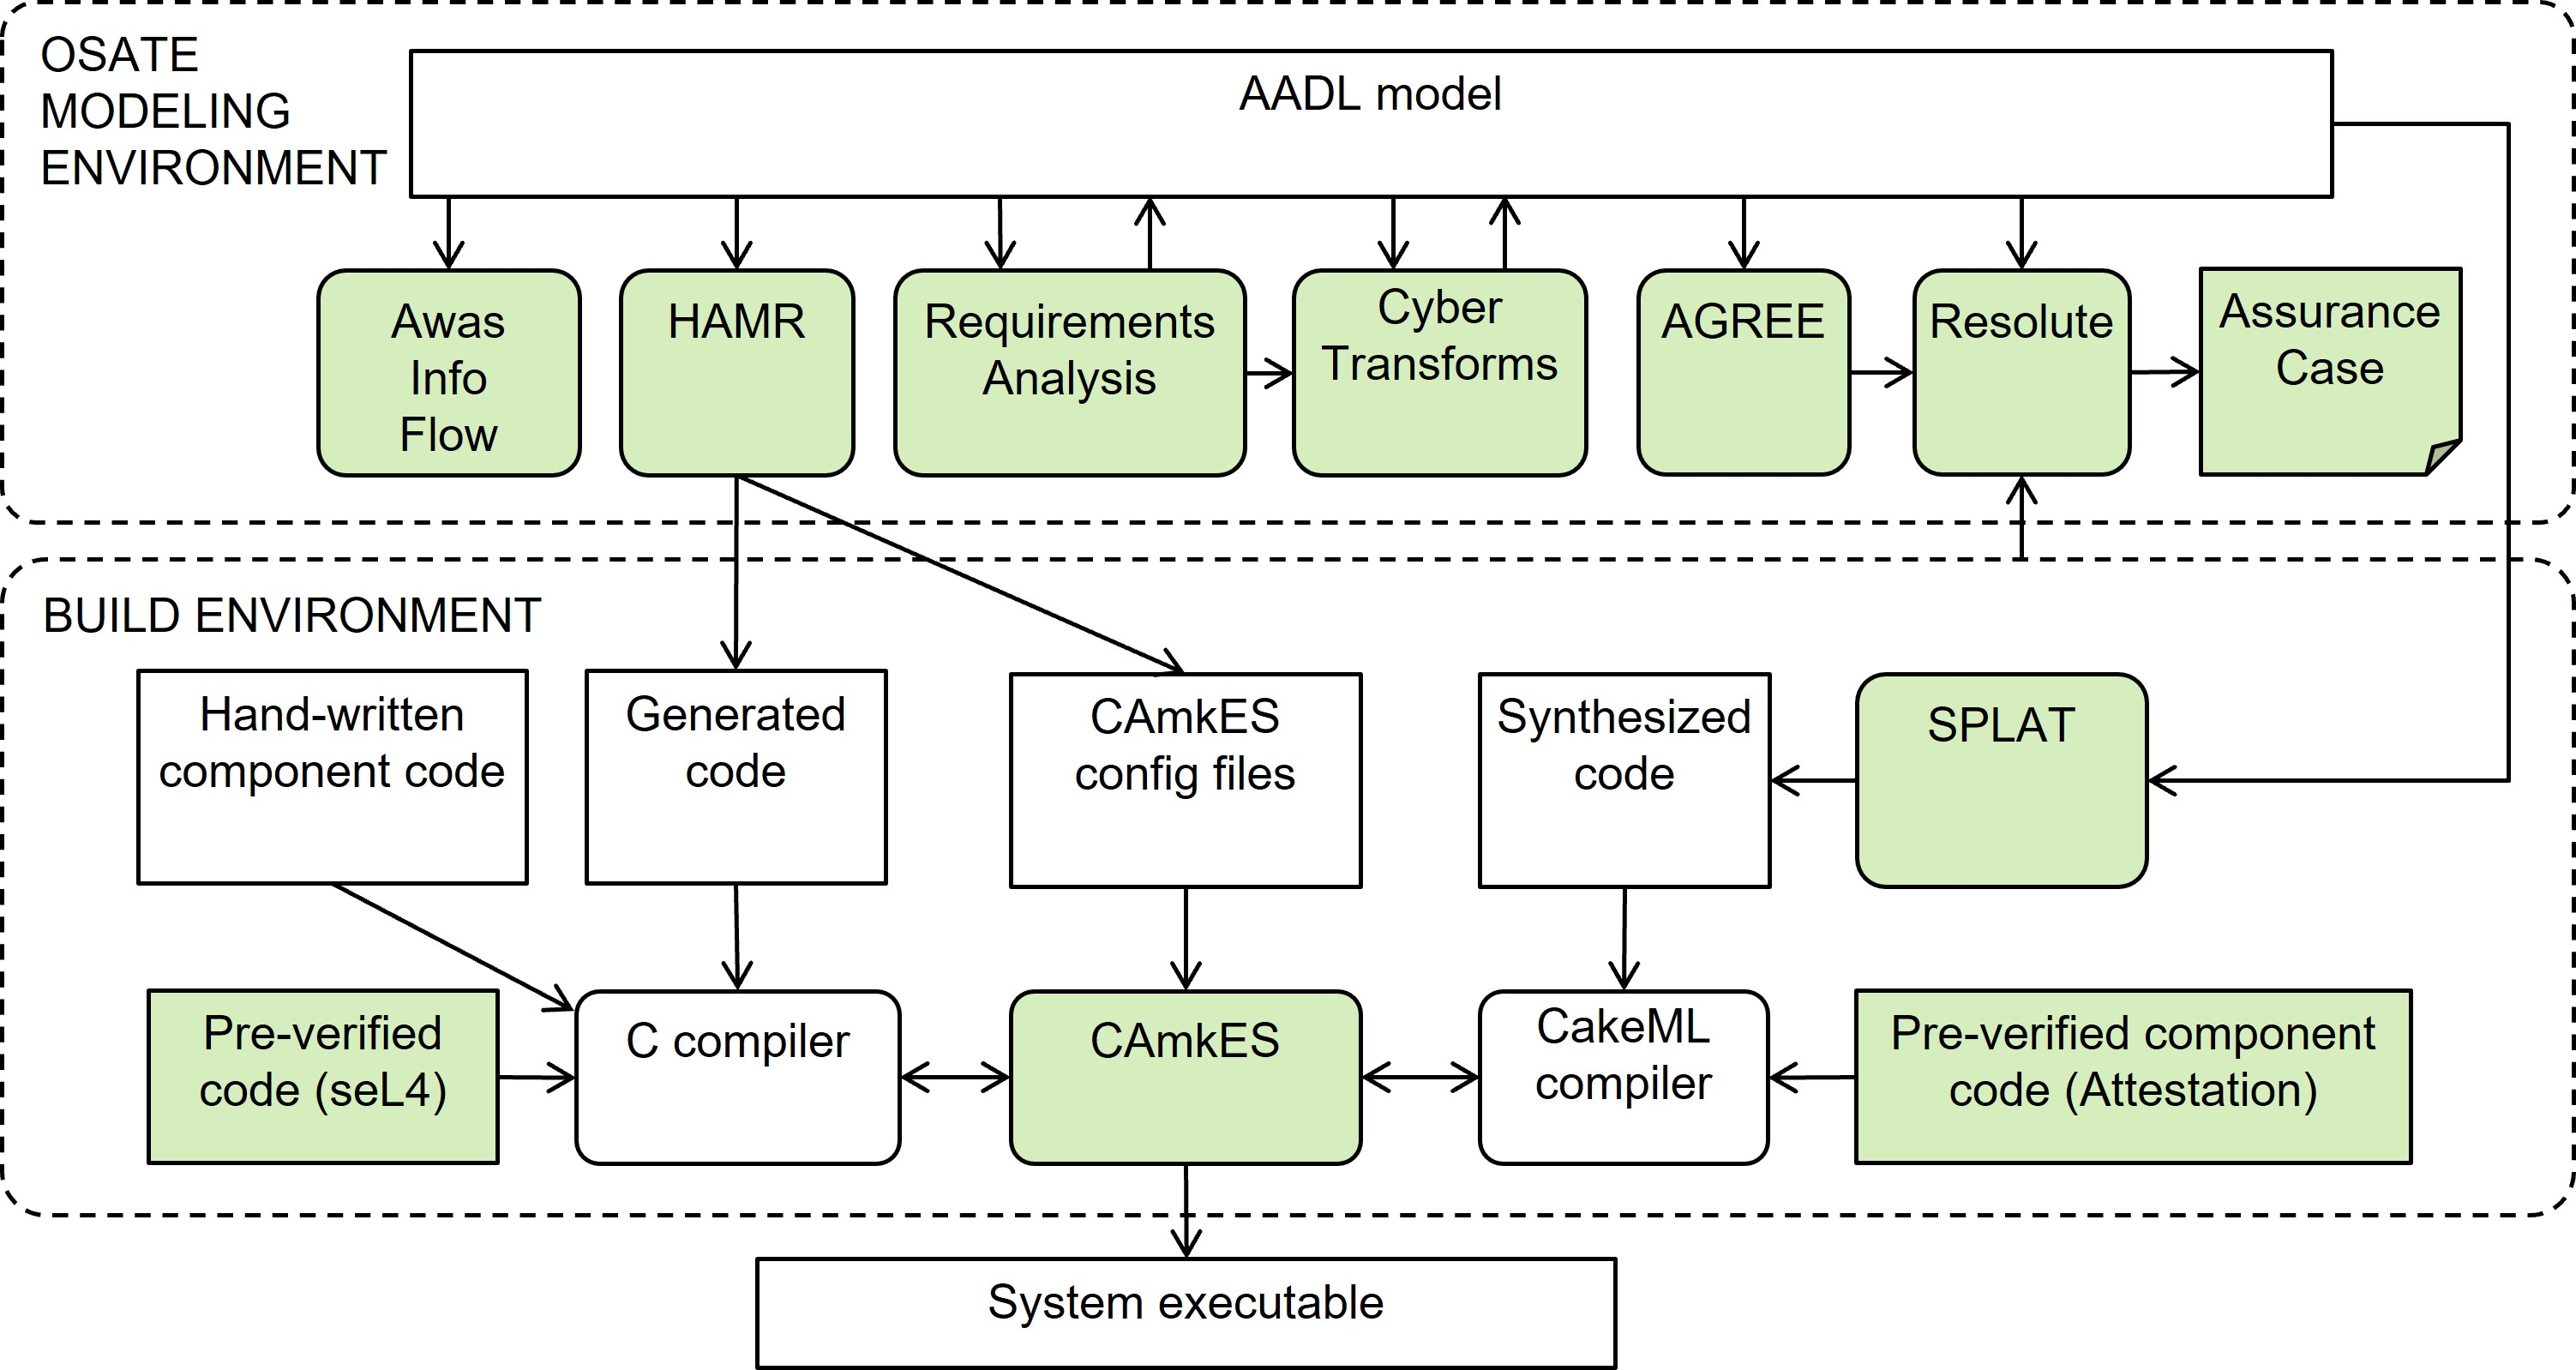
\includegraphics[width=\textwidth]{./figs/tool-arch.jpg}
  	\end{center}
	\caption{BriefCASE tool architecture.  Tools and code/artifacts discussed in the BriefCASE workflow are shown in green.} 
	\label{fig:tool-arch} 
\end{figure*}

\subsection{Requirements Analysis}

BriefCASE provides access to two analysis tools (GearCASE~\cite{gearcase2020} and
DCRYPPS~\cite{dcrypps2019}) that examine AADL models, report potential cyber vulnerabilities,
and suggest requirements for mitigation.
%
A BriefCASE project contains a repository for requirements. Imported requirements are represented 
as assurance case goals to be satisfied. 
The goal is marked {\em undeveloped} initially.
Evidential statements are added to the goal as the design is updated to address this requirement.
Some requirements are formalized as assume-guarantee contracts added to the AADL model.
Formal verification provides the evidence for the satisfaction of these requirements.

\subsection{Cyber Transforms}

To address the new cyber-resiliency requirement, the architecture will need to be transformed in such a way as to harden the design against the vulnerability.
BriefCASE provides an extendable library of model transformations for addressing common cyber vulnerabilities.  Currently, the following transformations are supported:

\begin{compactitem}
	\item Filter -- Blocks messages that do not conform to the given specification
	\item Monitor -- Detects violations of a given run-time condition and generates an alert
	\item Switch -- Used with a Monitor to block messages when an alert is generated (also referred to as a \textit{gate})
	\item Attestation -- Performs a measurement on non-local software to assess its trustworthiness
	\item Virtualization -- Isolates software component(s) in a virtual machine
	\item Proxy -- Inserts a pair of components to allow inspection of %https
		HTTPS message payloads
	\item seL4 -- Transforms the model to comply with seL4 component properties
\end{compactitem}  

The transformations are automated by the BriefCASE tool to create a hardened model that is correct-by-construction.  
These transformations include updates to the assurance case with new evidential statements indicating that the associated goal has been satisfied including the strategy used and links to context and associated evidence.  

\subsection{Compositional Analysis}

The Assume Guarantee Reasoning Environment (AGREE) is a compositional, assume-guarantee-style, model checker for AADL models \cite{compositional-analysis-agree}. 
AGREE attempts to prove properties about one layer of the architecture using properties allocated to subcomponents.
The composition is performed in terms of \emph{assumptions} and \emph{guarantees} that are provided for each component and from a \emph{contract} for the component.
Assumptions describe the expectations the component has on the environment while guarantees describe bounds on the behavior of the component.

The AGREE model checker verifies the \emph{consistency} of the composition of the component contracts.
\begin{compactenum}
\item Component interfaces -- The output guarantees of each component must be strong enough to
satisfy the input assumptions of downstream components. 
\item Correctness of implementations -- The input assumptions of a system along with the 
output guarantees of its \emph{sub}-components must be strong enough to satisfy its output guarantees.
\end{compactenum}
If the real-time schedule of the components for the deployed system is available, then AGREE is additionally able to generate an enhanced model that verifies the composition consistent under the schedule \cite{nfm:agree}.

\subsection{High Assurance Component Synthesis}

The correctness of the filter and monitors inserted by the BriefCASE transformations means that each such component must meet its AGREE contract.
This obligation is addressed by \emph{formal synthesis} using the Semantic Properties of Language
and Automata Theory (SPLAT) tool and is the topic of this paper.
SPLAT generates code to implement the AGREE contract and then proves that its implementation exactly preserves the meaning of the contract all the way down to the binary for the target platform \cite{case-models-2021}.

\subsection{Remote Attestation}

Semantic remote attestation is a technique for establishing trust in software running on a non-local computer.  
An appraiser requests an attestation from a target, receives evidence in response to the request, and appraises
the evidence to determine trust~\cite{Coker::Principles-of-R}.
Because remote attestation does not require modification of its measurement target, we utilize it to establish trust in legacy software that cannot otherwise be verified.
We construct a verified remote attestation infrastructure around the legacy target that generates run-time and boot-time evidence.

\subsection{Information Flow Analysis}

As systems become more complex, it is essential to have trustworthy methods to provide a common understanding of dependencies in the system and the respective responsibilities of the developers who may be from separate organizations.  
%
The Awas~\cite{awas} AADL information flow analyzer and visualizer has been applied to enable developers and auditors to understand, reason about, explore, and visualize system dependencies and information flows at scale across components and subsystems.
Awas processes the AADL system architecture model, specifically its inter-component connection descriptions and intra-component flow specifications, to provide formal system-wide impact and flow analyses.
Such flows include component data/control flows, security-oriented information flows, and fault/error propagation specified using the AADL Error Modeling Annex (EMv2).
Awas also provides a user-friendly Domain Specific Language (DSL) to query, check, and visualize custom safety or security system properties.

\subsection{Secure Microkernel}

The seL4 microkernel~\cite{sel4-sosp09} is a lightweight, fast, and secure operating system kernel.
Its implementation is fully formally verified, from high-level security properties down to the binary level.
It was the first OS kernel with this degree of formal verification, and after more than a decade of further research and engineering is still not only the leading formally verified OS kernel, but also the fastest OS kernel on the Arm architecture \cite{sel4-tocs14}. 

The true power of seL4 lies in its ability to scale formal analysis and verification to the much larger code bases that make up entire systems.
It does so by providing strong isolation between user-level components~\cite{sel4-cacm18}.
This isolation means that components can be analyzed separately from each other and be composed safely --- in this way seL4 provides the foundation that the soundness of the highly automated analysis tools such as AGREE depend on.
It makes it possible to run entire untrusted virtual machines and securely monitor their behavior on the
same hardware.
It makes it possible to provide filter and monitor components and prove that these components cannot be tampered with by the components they protect.
And it makes it possible to guarantee that the limited communication channels that the analysis tools assume to exist in the AADL model are the \emph{only} communication channels that are available to the
components in the system.
The combination of these enables automated high-level analysis with high assurance.

\subsection{Real-time Scheduling}

In mixed-criticality mission systems execution threads often have strict confidentiality, integrity, and availability requirements. 
\emph{Temporal isolation} is a secure technique to restrict timing channels and reduce temporal interference between software threads executing on the same platform. 
BriefCASE achieves temporal isolation through static cyclic scheduling using the sel4 domain scheduler.

BriefCASE generates a start-of-frame synchronization signal for each thread using a special thread called the \emph{Pacer}.
The Pacer sends periodic signals to each component thread.
Each component thread blocks until it receives its signal from the Pacer.
The thread then runs to completion and blocks again on the Pacer signal for the next iteration. 
Each thread subsequently executes exactly once during its statically scheduled time slice.

The new sel4 Mixed-Criticality Systems (MCS) variant provides additional capability that can support temporally isolated real-time systems. 
BriefCASE is also able to generate a static cyclic scheduler for MCS.
The MCS scheduler includes a start-of-frame signal so it eliminates the need for the Pacer component.
It also includes kernel level support for flexible dynamic scheduling.

\subsection{Infrastructure Code Generation}

The High Assurance Modeling and Rapid engineering for embedded systems tool (HAMR) is a multi-platform, multi-language AADL code generation framework \cite{hamr}. 
Using seL4 as a foundation, HAMR enables AADL to be used as a model-based development and systems engineering framework for seL4-based applications.
Its primary objectives is to support system builds that leverage seL4 separation and information flow guarantees to achieve the AADL-specified component isolation and inter-component communication needed for cyber-resiliency.
HAMR ensures that seL4 is configured to permit the exact inter-component information flows analyzed and visualized by Awas at the model level.

For each AADL thread component, HAMR generates a thread code skeleton and application programming interfaces (APIs) for communicating over the ports declared on the component.
For components that are implemented manually, the developer fills out the thread skeleton with application code.
HAMR supports coding component application logic in either C, Slang~\cite{slang} (a high-assurance subset of Scala that can be translated to C), or CakeML. 

HAMR generates component infrastructure and integration code implementing the semantics of AADL-compliant thread scheduling, thread dispatching, and port-based communication.
For port communication, shared memory communication (AADL data ports), buffered messaging (AADL event data ports), and buffered notification (AADL event ports) are supported.
HAMR code generation is staged using a translation architecture that facilitates adding new backends for different target platforms.
 
The seL4 deployment uses the component architecture for microkernel-based embedded systems (CAmkES) code-generation framework to configure the microkernel.
The HAMR generated CAmkES directly encodes the AADL model's component and communication topology and includes the AADL run-time infrastructure with its thread scheduling.
HAMR leverages the existing seL4 domain scheduler to enforce time partitioning and provide static cyclic scheduling.

HAMR also supports Linux-based virtual machine components in the seL4 deployment and the ability to run the entire system on the QEMU emulator.
HAMR automatically configures virtual machine based components, and this feature is used to sandbox the untrusted legacy code for the Mission Planner in the example UAV system.
The QEMU emulator support facilitates rapid prototyping for test, debug, and analysis, and it enables automated regression testing.

As part of its code generation process, HAMR produces flow graphs reflecting the inter-component information flow at both the AADL architecture level and the CAmkES level for the seL4 deployment.  
Visual representations are provided for manual inspection, and SMT-based representations are generated for formal reasoning.
The SMT-based representations are used to prove the following properties:
\begin{compactenum}
\item All AADL modeled flows are in the CAmkES configuration. 
\item No extraneous flows have been added to the CAmkES configuration.
\end{compactenum}
These properties focus on cyber-resiliency, but other key semantic properties can be verified as well.

\subsection{Assurance Case}

Assurance activities for high-integrity systems in the aerospace domain are currently driven by industry and government standards such as DO-178C and MIL-HDBK-516C.
The use of assurance cases to show conformance to standards (or provide alternate means of assurance) is being pursued in separate research programs.  
In addition, we have found that in assuring the cyber-resiliency properties of aircraft designs we need to integrate different kinds of evidence with varying levels of formality.
This has been our motivation for incorporating assurance case methods in BriefCASE.

In previous work, we developed the {\em Resolute} language and tool~\cite{resolute-destion} as a way to help engineers create an assurance argument describing the steps taken during the design process to make the system safe and secure.
The Resolute syntax supports construction of assurance cases that comply with the Goal Structuring
Notation (GSN) v2 standard.
Claims are expressed as \textit{goals} and \textit{strategies}, and can contain attributes such as \textit{context}, \textit{assumptions}, and \textit{justification}.
Claims can be marked \textit{undeveloped}, which Resolute interprets as an unsupported claim or with a \textit{solution}, which is an explicit assertion that the claim is supported.
Rather than being a separate document, a Resolute assurance case is part of the architecture model and can refer to elements within the model.
Since it is not a static representation, it can ensure that the assurance argument remains consistent with the evolving
design.  

BriefCASE includes a library of Resolute assurance strategies, or \emph{patterns}.
The patterns are instantiated with context from the AADL model and specify the evidence required to support the cyber-resiliency goals of the system.
For example, the \texttt{add\_filter} strategy is automatically inserted into the assurance case when the
\textit{Filter} transformation is performed, and it includes logical rules that Resolute uses to
determine whether its claim is supported by evidence.
\begin{compactitem} 
\item Component property implemented -- The filter has been implemented correctly 
to meet its AGREE specification as shown by the proof produced by SPLAT.
\item Filter is connected -- The filter component is still present at the correct location in the model and has not been altered or deleted by subsequent design changes. 
\item Filter cannot be bypassed -- There is no alternate information flow in the model that 
would allow the filter to be bypassed and therefore not perform its function.   
\item AGREE properties are valid -- The filter specification has been verified by AGREE to meet its
intended purpose in the system.   
\end{compactitem}